\section{Visual-Language Counter: End-to-End Framework for Zero-Shot Object Counting}
This section presents Visual-Language Counter~(VLCounter), an efficient end-to-end ZSOC framework.
We first establish a baseline model referred to as Vision-Language Baseline (VLBase), which exploits the visual-language localization capacity of CLIP in Sec.~\ref{Method:VLBase}.
Then, we bring three improvements on top of VLBase to introduce VLCounter.
Specifically, we emphasize the regions of interests~(Sec.~\ref{Method:SPT}), learn task-specific visual-language similarity~(Sec.~\ref{Method:LAT}), and exploit semantic-relevant information across the multi-level representations~(Sec.~\ref{Method:SaSC}).
The overall architectures of the two models are illustrated in Fig.~\ref{fig:VLCounter_overview}. 




\subsection{Visual-Language Baseline}
\label{Method:VLBase}
VLBase is a standalone baseline, eliminating the need for few-shot counting techniques that previous ZSOC approaches heavily rely on.
Given input query image $I$ and class name $C$, VLBase obtains patch embedding $\mathcal{V}$ and semantic embedding $\mathcal{T}$ using CLIP encoders $\phi_V(\cdot)$ and $\phi_T(\cdot)$, respectively.
By calculating the cosine similarity between $\mathcal{T}$ and $\mathcal{V}$, the similarity map $S\in \mathbb{R}^{H \times W}$ is yielded:
\begin{equation}
    S_{ij}(\mathcal{V},\mathcal{T}) = \frac{v_{ij}\mathcal{T}^\mathsf{T}}{||v_{ij}||||\mathcal{T}||},
\end{equation}
where $S_{ij}$ corresponds to the value at position $(i,j)$ in matrix $S$ and $v_{ij}$ represents the embedding at position $(i, j)$ of 2D-reshaped $\mathcal{V}$.



As mentioned in prior studies~\cite{2022maskclip, li2023clipsurgery}, we observed that the similarity map between CLIP-encoded semantic and patch embeddings provides an adequate indication of the degree of semantic similarity between the patch and semantic embedding.
We find that this similarity map is a decent clue for a decoder to localize the target objects.
Consequently, the CNN-based counting decoder predicts the density map $D_\text{pred}$ by utilizing features of $\mathcal{V}$ and $S$:
\begin{equation}
\label{eq3}
    D_\text{pred} = \phi_\text{decoder}([\mathcal{V}, S]),
\end{equation}
where $[\cdot,\cdot]$ denotes channel-wise concatenation.
Finally, the object count prediction is derived by summing all values in $D_\text{pred}$.



\paragraph{Counting Loss}
For training, we adopt a conventional MSE loss:
\begin{equation}
\label{eq3countingloss}
    \mathcal{L}_\text{count} = ||D_\text{pred} - D_\text{gt} ||^2_2,
\end{equation}
where $D_\text{gt}$ denotes the ground truth density map.



% SPT 모듈 그림
\begin{figure}[h]
    \begin{center}
    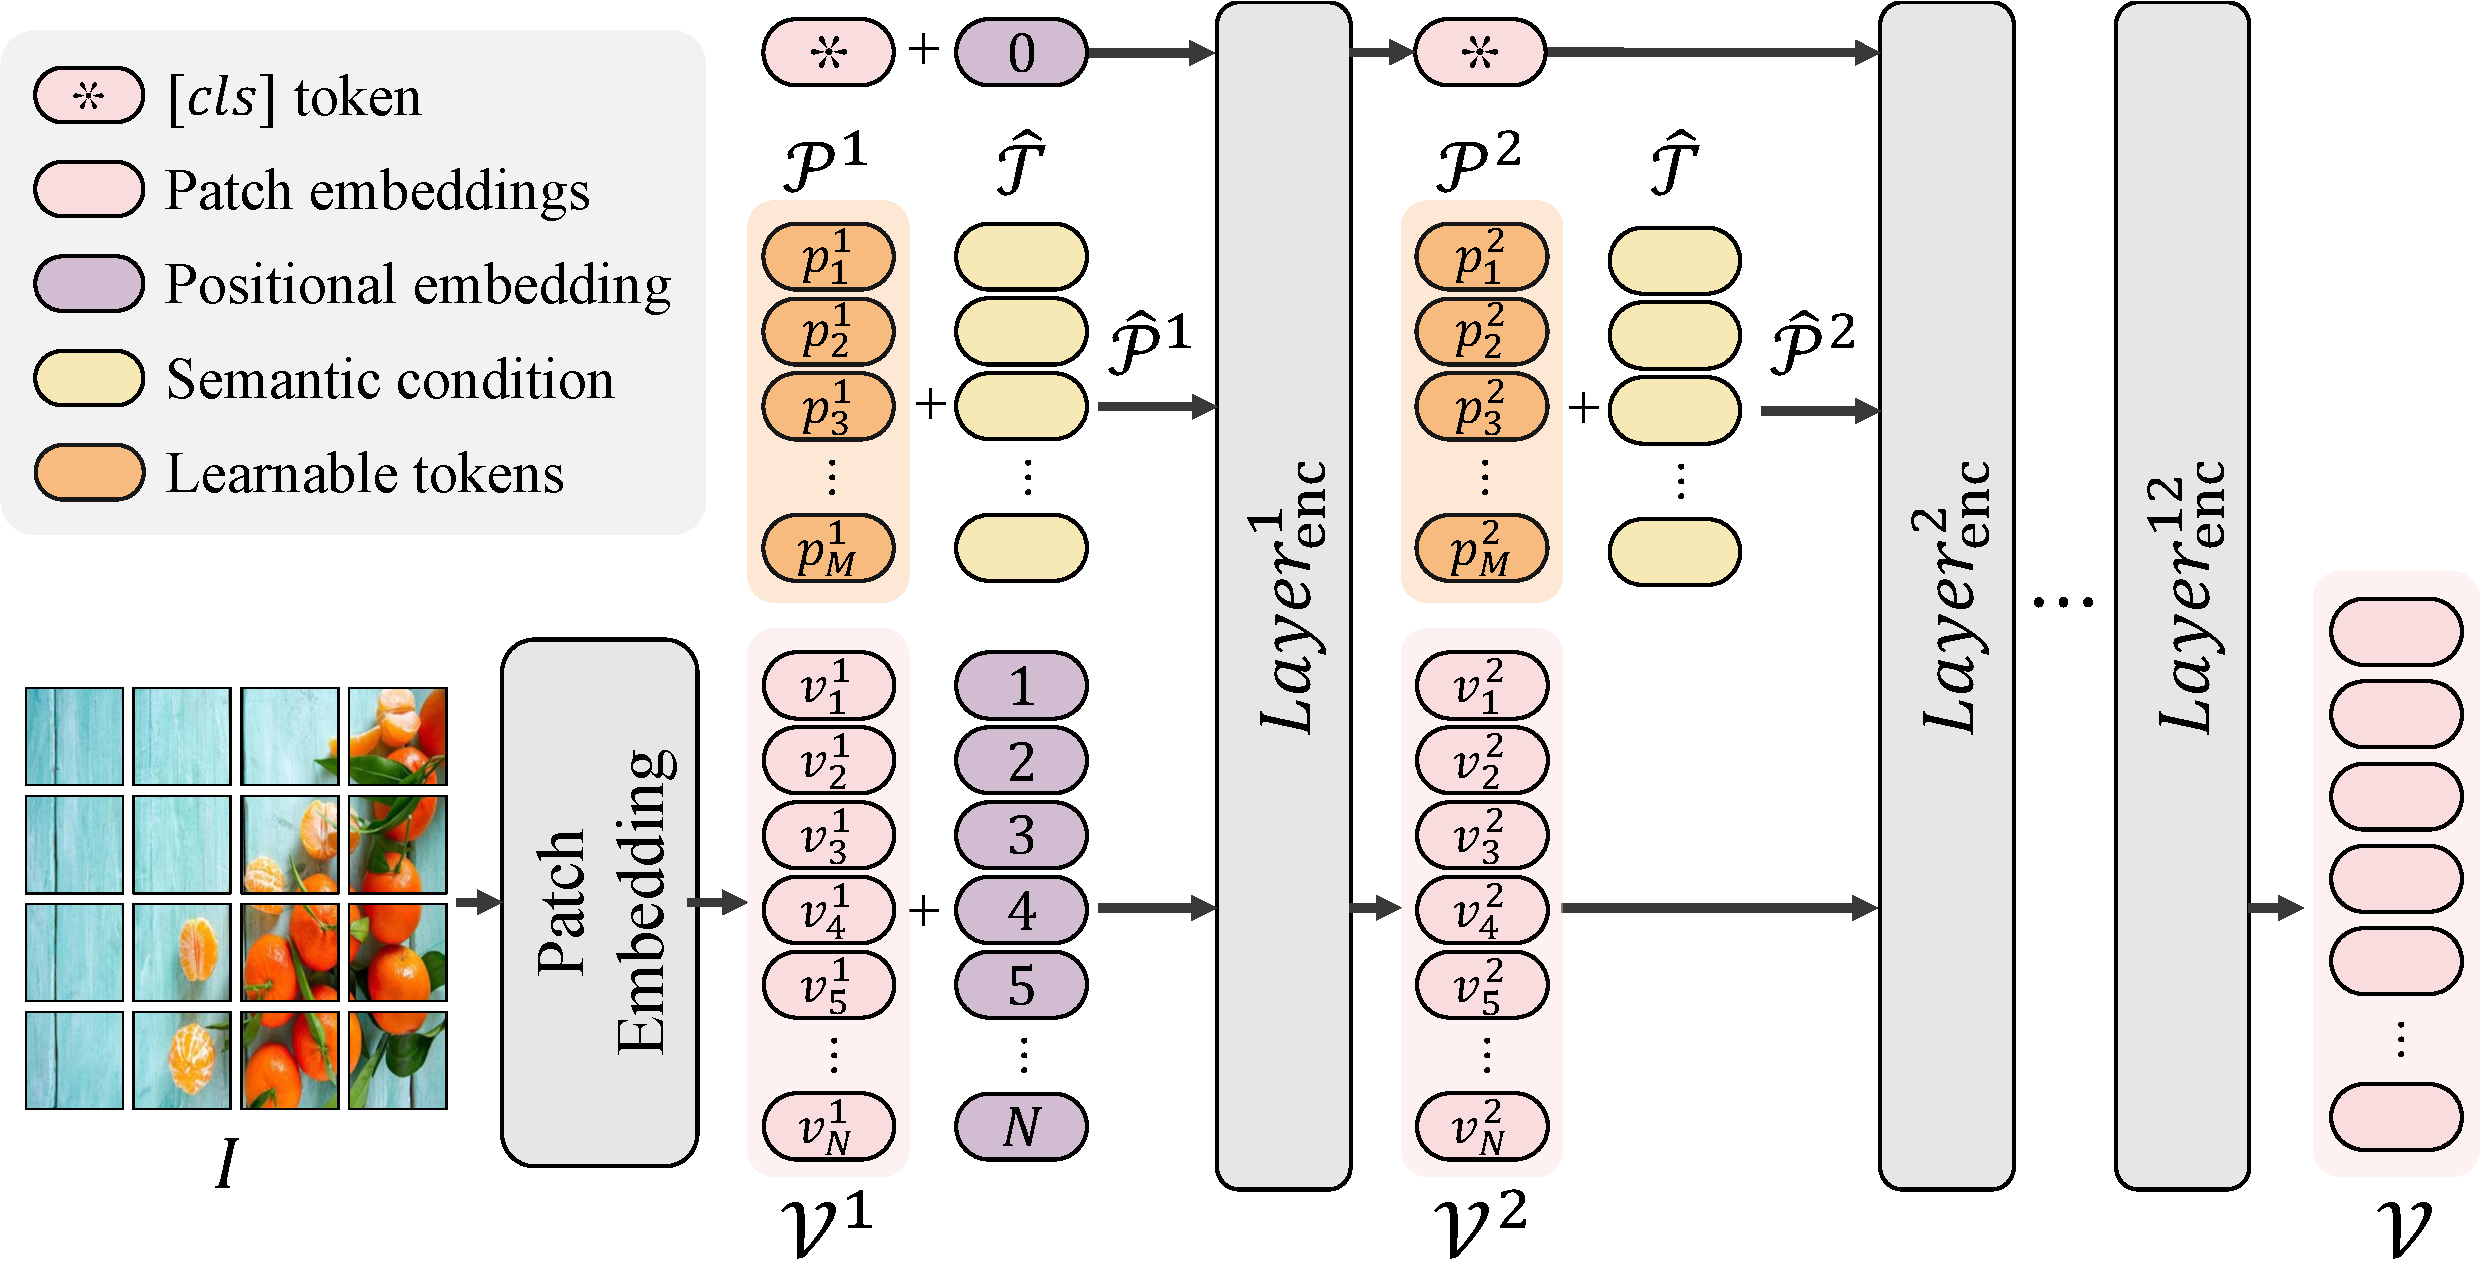
\includegraphics[width=\linewidth]{figs/SPT.pdf}
    \end{center}
    \caption{
        Illustration for Semantic-conditioned Prompt Tuning~(SPT).
        In addition to learnable visual prompts~(orange) in the image encoder, text features~(yellow) are integrated to specify the desired semantics.
    }
    \label{fig:SPT}
\end{figure}



\subsection{Semantic-conditioned Prompt Tuning~(SPT)}
\label{Method:SPT}
To grant task-specificity to the CLIP image encoder without sacrificing its generalization capability, a straightforward approach is to employ visual prompt tuning~(VPT)~\cite{2022vpt}.
However, the na\"ive VPT, which simply concatenates a few learnable tokens to the input sequence of each encoding layer does not take the semantic information into account.
Hence, we introduce Semantic-conditioned Prompt Tuning~(SPT), which utilizes semantic information along with the learnable tokens to assist the image encoder to extract target-semantic-highlighted visual features.


Specifically, as illustrated in Fig.~\ref{fig:SPT}, SPT has new learnable tokens for each encoding layer.
Learnable tokens for $l^{th}$ layer are defined as $\mathcal{P}^l = [p^l_1, p^l_2, ..., p^l_M]$ where the number of learnable tokens is denoted as $M$.
These tokens are then, supplemented with the linearly projected semantic embedding $\hat{\mathcal{T}}$ to generate semantic-conditioned prompts $\hat{\mathcal{P}}$.
The semantic-conditioned prompts for the $l^{th}$ layer are defined as follows:
\begin{equation}
    \hat{\mathcal{P}}^l = [p_1^l + \hat{\mathcal{T}}, p_2^l + \hat{\mathcal{T}}, p_M^l + \hat{\mathcal{T}}],
\end{equation}
where $\hat{\mathcal{T}} = \phi_c(\mathcal{T})$ and $\phi_c$ denotes the parameters of the projection layer.
Consequently, with the conditioned prompts $\hat{\mathcal{P}}$, the patch embedding process in $l^{th}$ layer of the image encoder can be expressed as:
\begin{equation}
    [\text{ }[cls],~\rule{0.25cm}{0.15mm},~\mathcal{V}^{l+1}\text{ }] = Layer^{l}_{\text{enc}}([\text{ }[cls],~\hat{\mathcal{P}}^{l},~\mathcal{V}^{l}\text{ }]),
\end{equation}
where initial input $\mathcal{V}^1=[v^1_1, v^1_2, \cdots, v^1_N]$ is a sequence of embedded patches through the patch embedding layer prior to the encoder.
Be aware that we follow VPT~\cite{2022vpt} to discard output tokens of $\hat{\mathcal{P}}$~(represented as $\rule{0.25cm}{0.15mm}$) and do not propagate to the subsequent layer.



\subsection{Learnable Affine Transformation~(LAT)}
\label{Method:LAT}
Through the adoption of the SPT, we obtain visual representations in which the corresponding regions of the target class are highlighted.
Nevertheless, due to the nature of object counting, discovering the central points of the objects rather than encompassing the entire object area, a discrepancy might arise between the information contained in the similarity map $S$ and the loss that needs to be backpropagated during training.


In light of this, we propose learnable affine transformation matrix~(LAT) to facilitate the conversion of similarity map $S$ to counting map $\hat{S}$ and establish a more task-specific visual-semantic linkage centered around individual objects as follows: 
\begin{equation}
    \hat{S} = W \otimes S + B,
\end{equation}
where $W, B \in \mathbb{R}^{H \times W}$ are learnable matrices for affine transformation and $\otimes$ indicates element-wise multiplication.
In addition, we directly optimize the counting map $\hat{S}$ with the rank-aware contrastive loss to learn the proper degree of activation for object counting. 
Details of rank-aware contrastive loss are elaborated in Sec.~\ref{Method:Loss}.
With LAT, the input to the decoder $[\mathcal{V}, S]$ in Eq.~\ref{eq3} of VLBase is replaced by $[\mathcal{V}, \hat{S}]$.



% SaSC 모듈 그림
\begin{figure}[t!]
    \begin{center}
    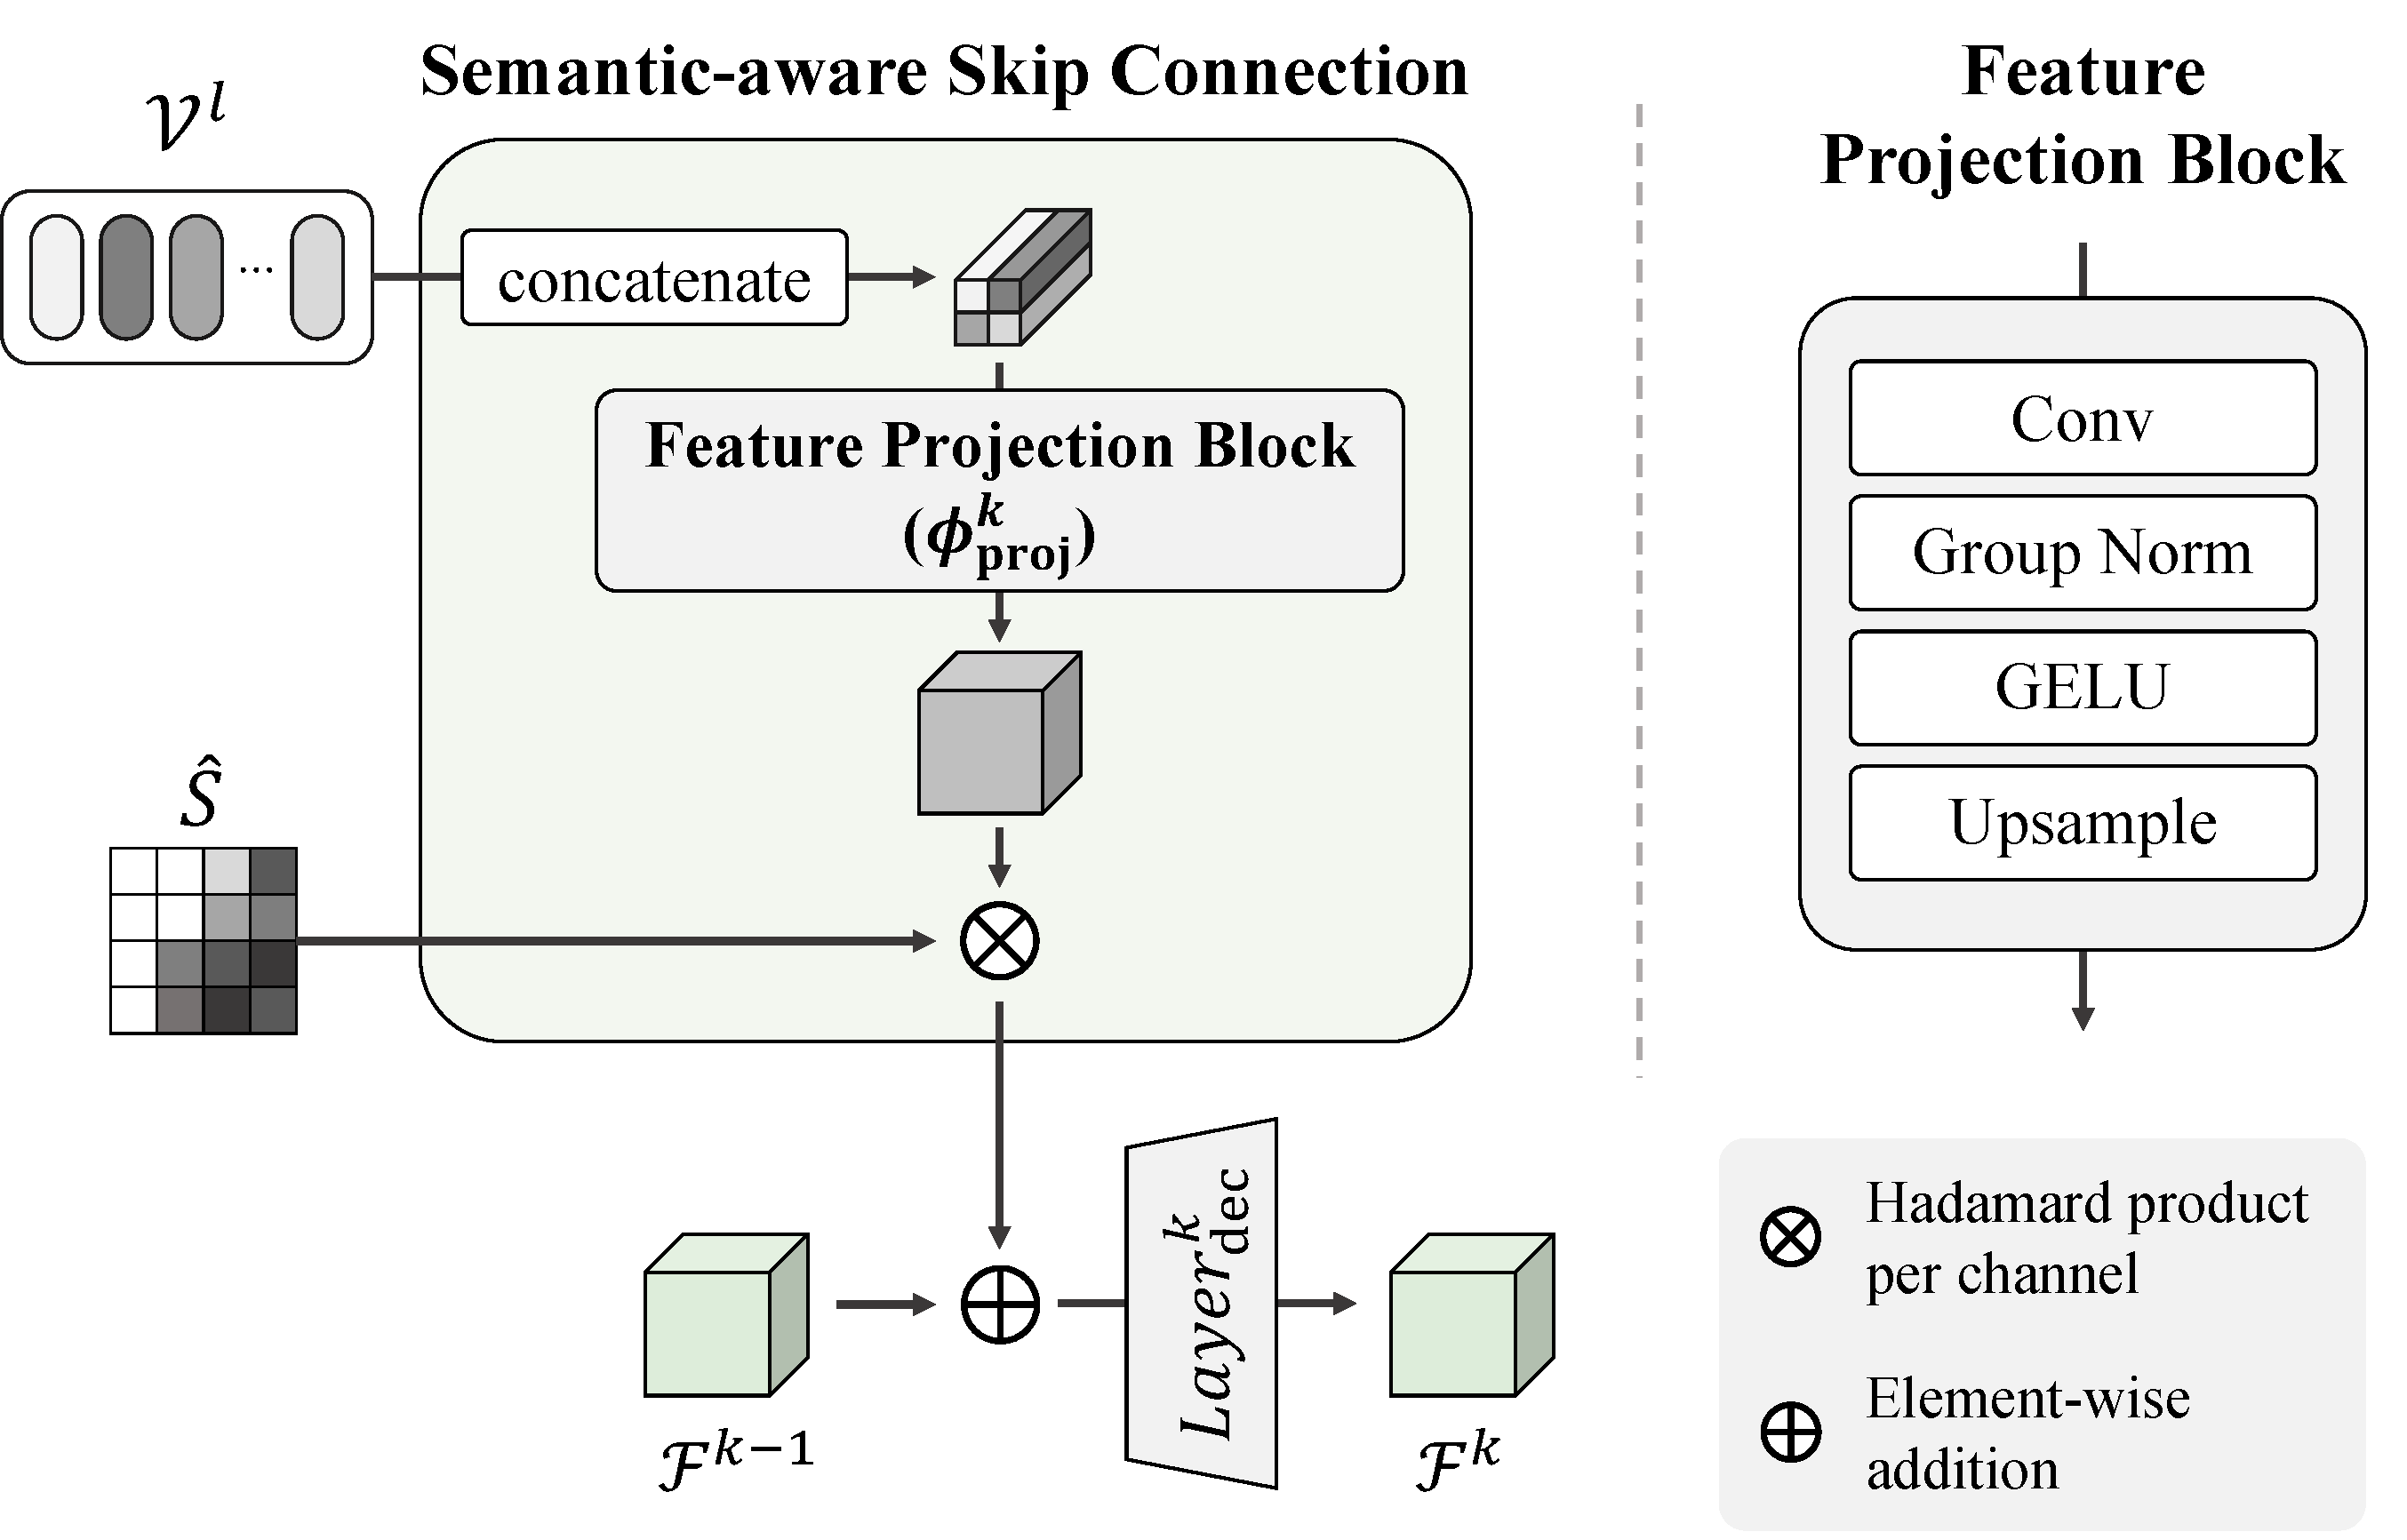
\includegraphics[width=\linewidth]{figs/SaSC.pdf}
    \end{center}
    \caption{
        The flow of Semantic-aware Skip Connection~(SaSC) and architecture of feature projection block.
        Intermediate visual features are projected and filtered with an object-aware counting map $\hat{S}$ to produce object-relevant encoder features. Consequently, these are integrated into its counterpart in the decoder.
    }
    \label{fig:SaSC}
\end{figure}



\subsection{Segment-aware Skip Connection~(SaSC)}
\label{Method:SaSC}
For ZSOC, where the model encounters unseen classes during inference, it is important to train a decoder that is tailored for object counting while maintaining a generalization ability.
Sharing the motivation with VLBase in Sec.~\ref{Method:VLBase} that CLIP features inherently preserve local semantics, we adopt skip connections that incorporate intermediate features of the encoder to its counterpart in the decoder.

\begin{table*}[t]
    \small
    \centering
    \setlength\tabcolsep{0pt}
    \setlength{\extrarowheight}{2.3pt}
    
    \begin{tabular*}{\textwidth}{@{\extracolsep{\fill}}*{1}{l} @{\extracolsep{\fill}}*{8}{c}}
    \hline

    % Header
    \multirow{2}{*}{Methods} & \multirow{2}{*}{Stage} & Class & \multirow{2}{*}{Train Dataset} & \multicolumn{2}{c}{Val set} & \multicolumn{2}{c}{Test set} & Inference \\%\multirow{2}{*}{inf.speed} \\
    \cline{5-6}\cline{7-8}
    & & Name & & MAE~$\downarrow$ & RMSE~$\downarrow$ & MAE~$\downarrow$ & RMSE~$\downarrow$ & speed~(s)~$\downarrow$\\
    \hline

    % Few-shot
    \textbf{\textit{few-shot}} & & & & & & \\
    GMN~\cite{2019GMN} & 1 & $\times$ & FSC147 & 29.66 & 89.81 & 26.52 & 124.57 & - \\
    FamNet~\cite{2021FAMNet} & 1 & $\times$ &FSC147 & 24.32 & 70.94 & 22.56 & 101.54 & 0.82 \\
    BMNet~\cite{2022BMNet} & 1 & $\times$ & FSC147 & 19.06 & 67.95 & 16.71 & 103.31 & 0.86 \\
    BMNet+~\cite{2022BMNet} & 1 & $\times$ & FSC147 & 15.74 & 58.53 & 14.62 & 91.83 & 1.59 \\
    \hline

    % Zero-shot
    \textbf{\textit{zero-shot}} & & & & & & & \\
    RepRPN-Counter~\cite{2022RepRPN} & 2 & $\times$ & FSC147~+~MS COCO~
    & 31.69 & 100.31 & 28.32 & 128.76 & - \\
    ZSC~\cite{2023zsc} & 2 & \checkmark & FSC147~+~MS COCO & 26.93 & 88.63 & 22.09 & 115.17 & 0.86+$\alpha$ \\
    VLBase~(Ours) & 1 & \checkmark & FSC147 & 31.82 & 98.89 & 32.20 & 130.51 & 0.81 \\
    VLCounter~(Ours) & 1 & \checkmark & FSC147 & \textbf{18.06} & \textbf{65.13} & \textbf{17.05} & \textbf{106.16} & 0.82 \\
    \hline
    
    \end{tabular*}
    \caption{
        Quantitative comparison to state-of-the-art approaches on the FSC147 dataset. 
        % GT stands for human-annotated boxes and Patch-Selection refers to selected patches with ZSC~\cite{2023zsc} approach.
        $\alpha$ in the rightmost column indicates an additional cost necessary for the exemplar discovery process in the context of the two-stage pipeline.
    }
    \label{tab:main}
\end{table*}


As shown in Fig.~\ref{fig:SaSC}, the $l^{th}$ encoder patch features are spatially concatenated and projected to yield decoder-assistive representations.
Then, we multiply the affine transformed similarity map $C$ to emphasize the object-relevant patches.
Finally, these patch features are added to the corresponding $k^{th}$ layer features of the decoder.
Formally, the $k^{th}$ decoding layer with SaSC, receiving $l^{th}$ encoder features, operates as follows:
\begin{equation}
    \mathcal{F}^{k} = Layer^{k}_\text{dec}(\mathcal{F}^{k-1} + \phi_\text{proj}^{k}(\mathcal{V}^{l}) \otimes \hat{S}),
\end{equation}
where $\phi_\text{proj}^{k}(\cdot)$, $\mathcal{F}^{k}$, and $\otimes$ stand for the parameter of feature projection block, the output of the $k$-th decoding layer, and Hadamard products per channel, respectively.


\subsection{Training Objectives}
\label{Method:Loss}
\Skip{
    To facilitate precise local visual-language alignment between patch embedding and semantic embedding
}
In addition to the counting loss described in Eq.~\ref{eq3countingloss}, VLCounter additionally employs rank-aware contrastive loss~\cite{hoffmann2022ranking, moon2023query}.
Whereas the $\mathcal{L}_{\text{count}}$ trains the whole model to learn the counting objective, 
our focus in SPT and LAT is learning to yield the counting-tailored similarity map in the encoder.
In this regard, we adopt rank-aware contrastive loss in the counting map $\hat{S}$ to assign higher activations on the patches that are nearby the object centers.
To design the hierarchical guidance for a rank-aware contrastive loss, we first normalize the ground truth density map $D_{\text{gt}}$ to be mapped between 0 and 1.
Then, we iterate the batch for $K$ times with different thresholds to prepare positive and negative sets; patches are gathered as positive if the corresponding patch in $D_\text{gt}$ has a higher value than the threshold, and if not, as negative.
Formally, the rank contrastive loss with the positive set $\hat{S}_r^\text{pos}$ and the negative set $\hat{S}_r^\text{neg}$ is formulated as follows:
\begin{eqnarray}
    \label{eq7contrastiveloss}
    \mathcal{L}_{\text{rank}}=-\sum_{k=1}^{K}\text{log}\frac{
    \sum_{\hat{S}_i\in \hat{S}_r^\text{pos}}\text{exp}(\hat{S}_i/\tau)}
    {
    \sum_{\hat{S}_j\in (\hat{S}_r^\text{pos} \cup \hat{S}_r^\text{neg})}\text{exp}(\hat{S}_j/\tau)
    },
\end{eqnarray}
where $\tau$ is a temperature scaling parameter.


With the objectives in Eq.~\ref{eq3countingloss} and Eq.~\ref{eq7contrastiveloss} combined, VLCounter's final objective is as follows:
\begin{equation}
    \mathcal{L}_{\text{total}} = \mathcal{L}_{\text{count}} + \lambda \cdot \mathcal{L}_{\text{rank}},
\end{equation}
where $\lambda$ is a hyperparameter to balance between the losses.